
\chapter{QUIC Protocol}\label{chap:02-quic}

This chapter is intended as a summary of the QUIC protocol specification providing sufficent detail
for the design of our implementation. The text is based on the version 29 of the draft specification
documents from June 2020, more specifically on the documents describing the core transport
protocol~\cite{draft-ietf-quic-transport}, TLS integration~\cite{draft-ietf-quic-tls}, and
congestion control mechanism~\cite{draft-ietf-quic-recovery}. Readers familiar with these documents
may skip this chapter.

We will start this chapter by first providing a high-level overview of QUIC, and then provide a more
detailed description of individual parts of the protocol.

\section{Overview of QUIC}

QUIC protocol provides a reliable and secure transport of multiple streams of data over a single
connection\footnote{The ability to transport multiple streams over a single connection is called
  \textit{stream multiplexing}}. QUIC is implemented on top of UDP, which provides only unreliable
transfer of datagrams. Stream multiplexing, loss recovery, congestion control, security and other
features known from TCP or TLS, respectively, are implemented by QUIC itself.

\subsection{QUIC Connection}
As in other protocols, QUIC allows communication between two endpoints: client and server. In QUIC
connection, endpoints exchange QUIC packets. A single UDP datagram can contain multiple packets,
although it generally contains only one. Bundling multiple QUIC packets in a single UDP datagram is
called \textit{coalescing}. QUIC packets cannot span multiple UDP datagrams. The QUIC connection is
identified by its Connection ID\@. \todo{decide if we want to use special font for things like
  Connection ID, Stream ID, etc.} During connection establishment, each peer choses the \todo{verify
  if there should be indefinite article or not} Connection ID which the other endpoint should
include in the header of sent packets in the \textit{Destination Connection ID} (DCID for short)
\todo{list all abbreviations at the end/beginning of the thesis?}.

The separation of connection identity from the used socket allows multiple connections to be made
using the same socket. \autoref{fig:02-connection-multiplexing} illustrates how the incoming
packets are associated with individual connections based on the DCID field of the packet header.

\begin{myFigure}{fig:02-connection-multiplexing}{Multiple QUIC connections on the same machine port}
  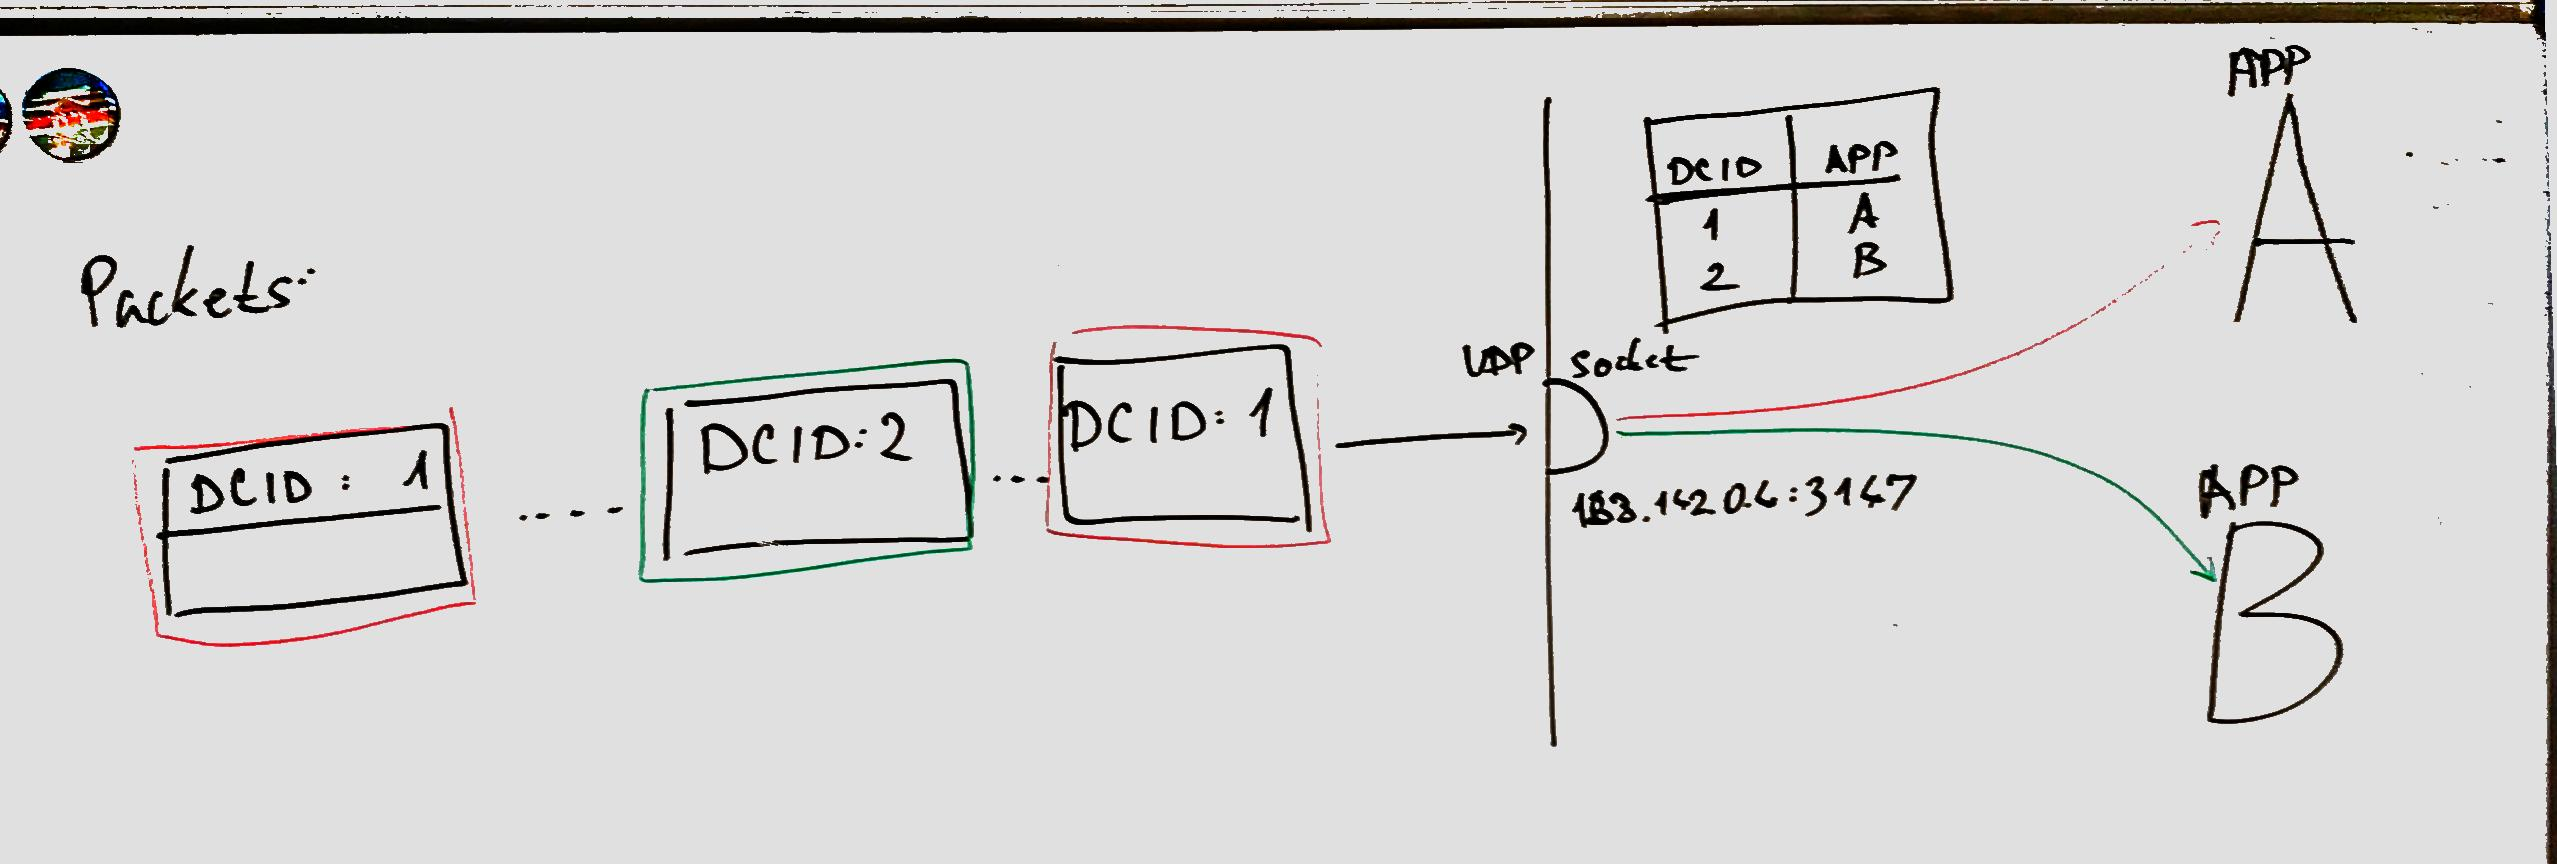
\includegraphics[width=0.9\textwidth]{img/02-socket-multiplexing}
\end{myFigure}

\todo{better describe the image, it is hard to decypher, TODO, really different applications?}

\subsection{QUIC Packets}

QUIC packets sent in the UDP datagram are the smallest processible unit of QUIC\@. The packets are
formed by a header and variable-length payload consisting of one or more QUIC frames. QUIC frames
carry individual pieces of information such as acknowledgements or parts of the streams sent by
the application.

Similarly to TCP, packets in QUIC connections are numbered. However, QUIC uses three separate
\textit{Packet number spaces}:

\begin{enumerate}
  \litem{Initial} Used for exchanging initial information.
  \litem{Handshake} Used during the connection handshake process.
  \litem{1-RTT} Used throughout the lifetime of the connection to transfer application data.
\end{enumerate}

Packets from each packet number space are numbered and processed independently of the other packet
spaces. This includes also acknowledgements for received packets. Acknowledgement for an Initial packet can be sent only in another Initial packet and vice versa.

\subsection{Packet Encryption}

QUIC packets are encrypted by a symmetric cryptographic cipher. Each packet number space uses
different keys for packet encryption. Initial keys are derived using only the Connection ID chosen
by the client and therefore provide just an obfuscation. Handshake keys are intermediate protection
keys derived during TLS handshake. 1-RTT keys are negotiated by the TLS 1.3 protocol and offer the
same level of security as standard TLS 1.3 connection. The packet encryption is used for protection
both against network traffic observers and against packet payload corruption.

\subsection{Stream Multiplexing}

QUIC can transport multiple streams of data in a single connection. Each stream can be either
unidirectional or bidirectional, and is identified by its Stream ID. Each streamand is processed
independently of the other streams. \autoref{fig:02-stream-multiplexing} illustrates how QUIC may
pack two streams into frames such that those streams are transported in parallel.

\begin{myFigure}{fig:02-stream-multiplexing}{Stream multiplexing in QUIC}
  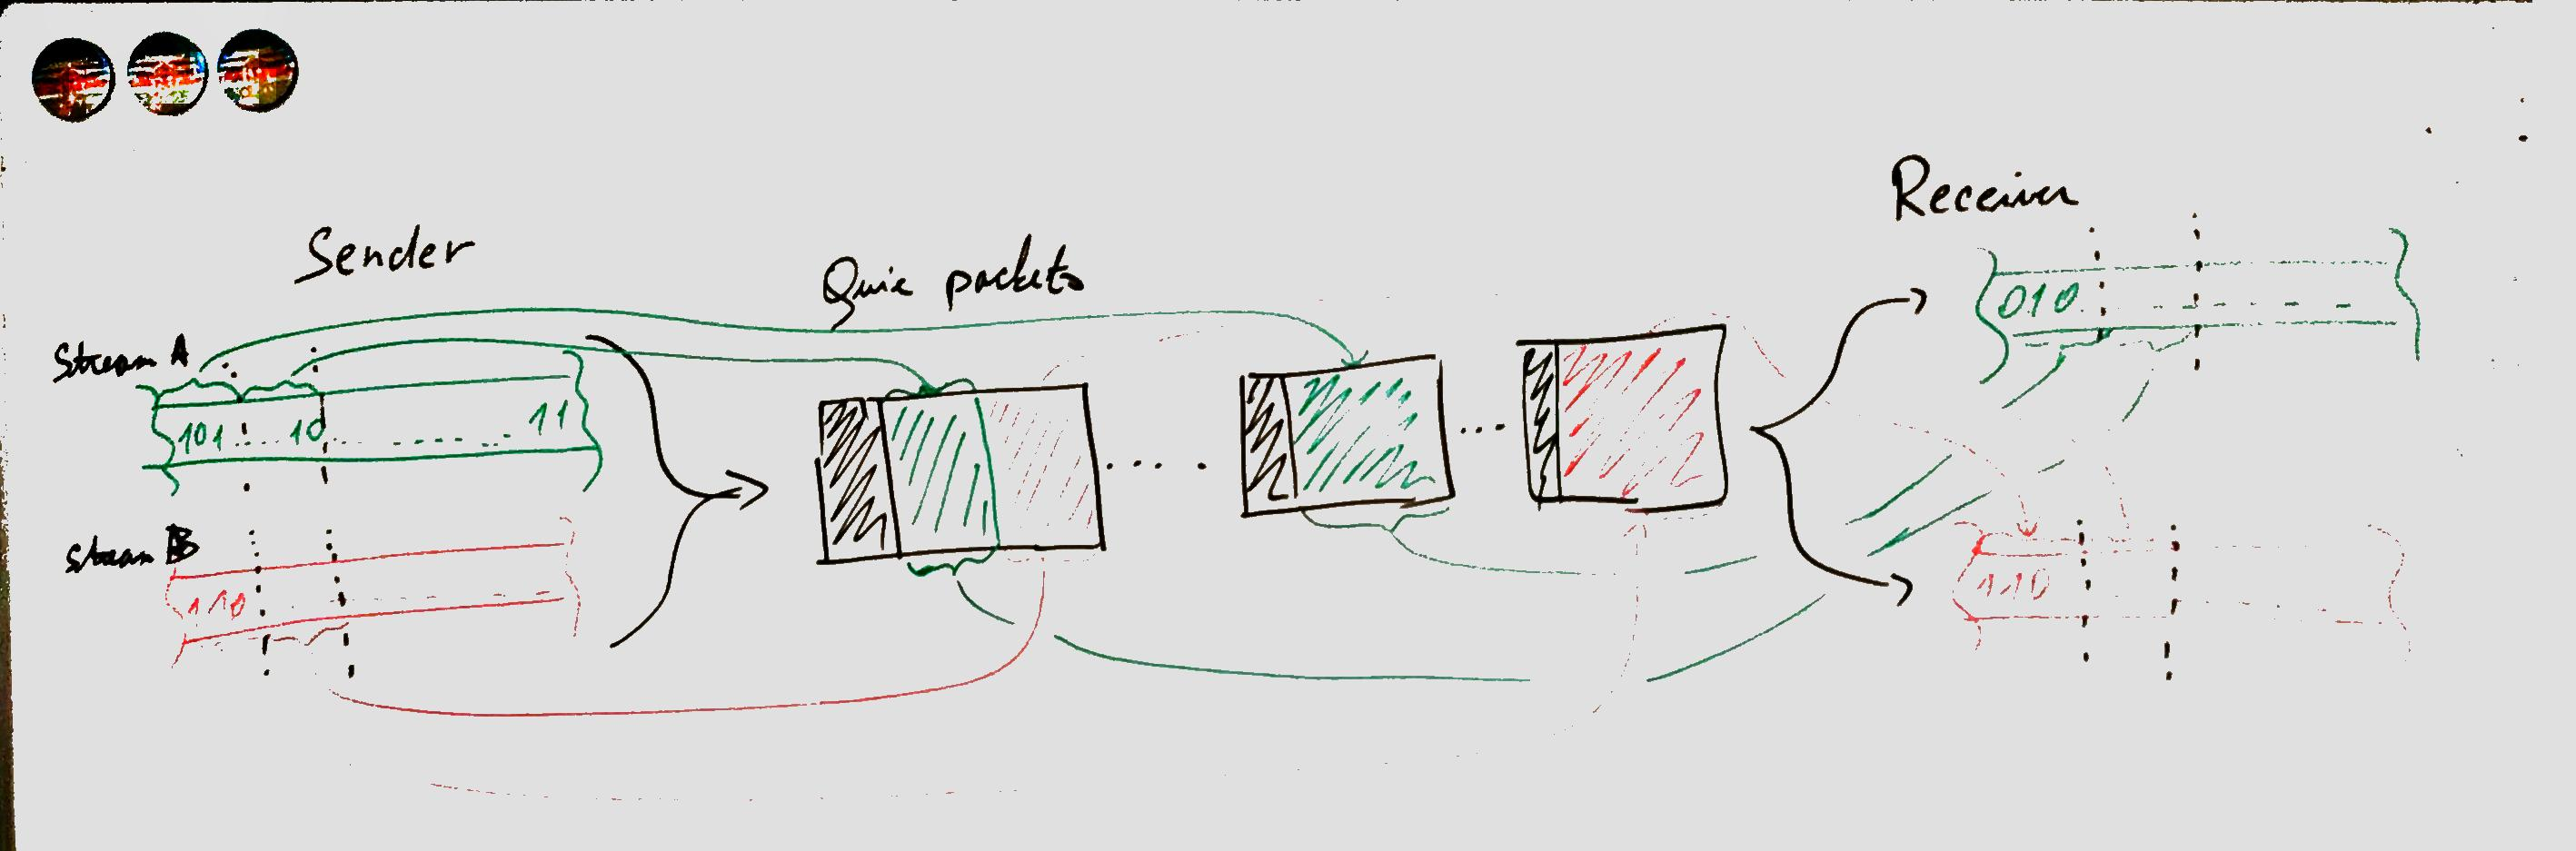
\includegraphics[width=0.9\textwidth]{img/02-stream-multiplexing}
\end{myFigure}

\todo{change the picture so that the newest data is on the right side, basically just flip the
  stream on the Sender's side}

\subsection{Flow Control}

As a prevention against malicious too fast senders, QUIC implements a credit based flow-control
scheme. In this scheme, each peer advertises how much data it is willing to accept and how many
streams of each type can be opened by its peer.

\subsection{Loss Detection and Recovery}

Becuase UDP is an unreliable transport protocol, and QUIC must detect loss of the packets sent. The
loss detection is implemented similarly to TPC via acknowledgements of the received packets.
However, an important difference from TCP is that the lost packet is not retransmitted as-is.
Instead, each QUIC frame in the original packet is either updated and sent in some future packet, or
--- if the information is no longer relevant --- dropped altogether.

\autoref{fig:02-packet-loss-example} illustrates the retransmission process. When the sender
receives acknowledgement for packet 3, it infers that packet 2 never reached the receiver, and
retransmits the STREAM frame in packet 4. The ACK frame for packet 1 does not need to be
retransmitted, because it was sent in packet 3. Therefore, packet 4 includes ACK only for packet 2.

\todo{redraw the image to match the description above}

\begin{myFigure}{fig:02-packet-loss-example}{Retransmission of lost data in QUIC}
  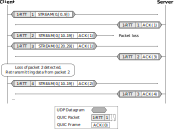
\includegraphics[width=0.5\textwidth]{img/02-retransmission-example}
\end{myFigure}

\todo{if the image is deleted then the text should still make sense! I must add description what I
  actually see on the image. Also, make the image more like a UML process diagram}

\subsection{Wire Encoding}

The process of encoding QUIC packets to be sent via the network is optimized for size. All values
sent over the network are encoded in Big-Endian, also known as \textit{network order}. Almost all
numerical values are encoded using a variable-length integer encoding. This encoding uses the two
most significant bits of the first byte to encode whether the value is encoded as 1, 2, 4 or 8 byte
integer. This encoding supports only positive numbers. The ranges available for individual encoding
lengths are listed in \autoref{tab:02-quic-varint-length}.

\begin{myTable}
  {tab:02-quic-varint-length}
  {Variable-length integer encoding lengths}
  {ccr}
  {Most significant bits & Encoding length (B) & Maximum value}
    00                   & 1                   & \num{63}         \\
    01                   & 2                   & \num{16383}      \\
    10                   & 4                   & \num{1073741824} \\
    11                   & 8                   & $2^{62}-1$       \\
\end{myTable}

In order to optimize the size of QUIC packets, the implementations should choose the smallest
possible encoding possible for each encoded number.

\section{QUIC Connection}

In the overview section, we mentioned that QUIC Connections are identified by Connection ID and that
QUIC Packets are exchanged between the endpoints. There are total of five different packet types
that are used in QUIC\@:

\begin{enumerate}
    \litem{Initial \textnormal{and} Handshake} used during connection establishment;

    \litem{1-RTT} main packets used during the lifetime of QUIC connection;

    \litem{Version Negotiation} sent by server when client tries to establish connection using
    unsupported version of QUIC\@;

    \litem{0-RTT} carries \textit{early data} when TLS 1.3 0-RTT mode of operation is enabled; and

    \litem{Retry} optionally used by servers for client's address validation when establishing new connections.
\end{enumerate}

Initial, Handshake and 1-RTT packets correspond to the three packet number spaces used throughout
the connection lifetime. For packet processing purposes like acknowledgements and loss detetion, the
1-RTT packet number space also includes 0-RTT packets. Version Negotiation and Retry packets are
used in special cases, are not associated with a packet number space and therefore are neither
encrypted or numbered.

\subsection{QUIC Frames}

Packets of type Initial, Handshake, 0-RTT and 1-RTT packets carry low-level QUIC protocol messages
called QUIC frames. These include e.g.\ ACK frames carrying acknowledgements for received packets,
STREAM frames carrying application data, and CRYPTO frames carrying data for TLS handshake.

All received QUIC packets have to be acknowledged. However, the frame types carried in the packet
determine whether the receiver must acknowledge it immediately or later when it sends some data on
its own. For example, packets containing only ACK frames are not acknowledged immediately to avoid
unnecessary traffic. Frame types requiring immediate ack are called \textit{ack-eliciting frames},
and the packets with at least one such frame are called \textit{ack-eliciting packets}.

There are also restrictions on which frames can be sent in which packets. For example, the STREAM
frames can only be sent in an 1-RTT frames to avoid compromising security.
\autoref{tab:02-frame-types} lists all frame types, whether they are ack-eliciting and in which
packets they can be sent.

\begin{myTable}[\small]
  {tab:02-frame-types}
  {QUIC frame types}
  {l@{\hskip -0.1in}ccccc}
  {                    &               & \multicolumn{4}{c}{Allowed in packet type}                \\ \cmidrule(lr){3-6}
   Frame type          & Ack-eliciting & Initial      & Handshake    & 0-RTT        & 1-RTT}
PADDING                &               & \checkmark{} & \checkmark{} & \checkmark{} & \checkmark{} \\
PING                   & \checkmark{}  & \checkmark{} & \checkmark{} & \checkmark{} & \checkmark{} \\
ACK                    &               & \checkmark{} & \checkmark{} &              & \checkmark{} \\
RESET\_STREAM          & \checkmark{}  &              &              & \checkmark{} & \checkmark{} \\
STOP\_SENDING          & \checkmark{}  &              &              & \checkmark{} & \checkmark{} \\
CRYPTO                 & \checkmark{}  & \checkmark{} & \checkmark{} &              & \checkmark{} \\
NEW\_TOKEN             & \checkmark{}  &              &              &              & \checkmark{} \\
STREAM                 & \checkmark{}  &              &              & \checkmark{} & \checkmark{} \\
MAX\_DATA              & \checkmark{}  &              &              & \checkmark{} & \checkmark{} \\
MAX\_STREAM\_DATA      & \checkmark{}  &              &              & \checkmark{} & \checkmark{} \\
MAX\_STREAMS           & \checkmark{}  &              &              & \checkmark{} & \checkmark{} \\
DATA\_BLOCKED          & \checkmark{}  &              &              & \checkmark{} & \checkmark{} \\
STREAM\_DATA\_BLOCKED  & \checkmark{}  &              &              & \checkmark{} & \checkmark{} \\
STREAMS\_BLOCKED       & \checkmark{}  &              &              & \checkmark{} & \checkmark{} \\
NEW\_CONNECTION\_ID    & \checkmark{}  &              &              & \checkmark{} & \checkmark{} \\
RETIRE\_CONNECTION\_ID & \checkmark{}  &              &              & \checkmark{} & \checkmark{} \\
PATH\_CHALLENGE        & \checkmark{}  &              &              & \checkmark{} & \checkmark{} \\
PATH\_RESPONSE         & \checkmark{}  &              &              & \checkmark{} & \checkmark{} \\
CONNECTION\_CLOSE      &               & \checkmark{} & \checkmark{} & \checkmark{} & \checkmark{} \\
HANDSHAKE\_DONE        & \checkmark{}  &              &              &              & \checkmark{} \\
\end{myTable}

\subsection{Connection Establishment}

QUIC connection is considered establishmed when the TLS handshake is completed. This implies that
both peers have derived the necessary protection keys to be able to receive application data carried
in 1-RTT frames.

An example handshake flow is illustrated in
\autoref{fig:02-example-handshake-flow}. The figure lists also the semantics of the content of the
CRYPTO frames sent. However, this is only for illustrative purposes as QUIC does not interpret the
contents of the CRYPTO frames.

\begin{myFigure}
  {fig:02-example-handshake-flow}
  {Example QUIC handshake flow}

  \begin{verbatim}
   Client                                                  Server

   Initial[0]: CRYPTO[CH] ->

                                    Initial[0]: CRYPTO[SH] ACK[0]
                          Handshake[0]: CRYPTO[EE, CERT, CV, FIN]
                                    <- 1-RTT[0]: STREAM[1, "..."]

   Initial[1]: ACK[0]
   Handshake[0]: CRYPTO[FIN], ACK[0]
   1-RTT[0]: STREAM[0, "..."], ACK[0] ->

                               1-RTT[1]: STREAM[3, "..."], ACK[0]
                                          <- Handshake[1]: ACK[0]
  \end{verbatim}
  \todo{Note that this is copied from RFC? Also, this example lacks the HANDSHAKE\_DONE frame}

  \todo{Make this diagram graphical, not textual}
\end{myFigure}

In it's first datagram, client sends an Initial packet with a single CRYPTO frame contaiting the
\textit{Client Hello} TLS message.

Server replies with a datagram containing three coalesced QUIC packets. The first is an Initial
packet that acknowledgement for the clients Initial packet, and a CRYPTO frame with a \textit{Server
  Hello} message. The contents of the Client Hello are then used to derive Handshake protection keys
and more TLS messages can be sent in the CRYPTO frame in the Handshake packet. The server also has
enough information to derive the 1-RTT keys, so it can also start sending data on Stream 1 using the
STREAM frame in a 1-RTT packet.

Because the servers Initial packet contained an ack-eliciting CRYPTO frame, client needs respond
with another Initial frame with an ACK frame. Contents of the Server Hello message allow client to
derive Handshake protection keys and process the servers Handshake packet. The Handshake packet
needs to be separately acknowledged by an ACK frame and a reply from the TLS layer must be sent in
another CRYPTO frame. By this time, client can also derive 1-RTT protection keys and send or receive
application data in STREAM frames.

\subsection{Connection Termination}

QUIC connection can be terminated in three ways:

\begin{itemize}
  \item Idle timeout
  \item Immediate close
  \item Stateless reset
\end{itemize}

\subsubsection{Idle Timeout}

If idle timeout is enabled, the connection is silently closed if no packet from the peer has been
received for the specified period of time. Each peer may advertise a \texttt{max\_idle\_timeout}
transport parameter, but the effective value is the minimum of the two values.

To prevent timeouts endpoints can send a PING or another ack-eliciting frame to test the liveness of
the connection. However, sending of PING frames should be initiated by the application protocol, not
QUIC implementation itself to prevent sending unnecessary PING frames.

\subsubsection{Immediate close}

Immediate close can be initiated both by QUIC implementation and by the application protocol. An
endpoint can initiate an immediate close by sending a CONNECTION\_CLOSE frame. This causes all
streams to immediately become closed.

By sending a CONNECTION\_CLOSE frame, the peer enters a closing state, in which it includes the
CONNECTION\_CLOSE frame in all packets it sends in reply to incoming packets.

Upon receiving a CONNECTION\_CLOSE, the peer should echo the CONNECTION\_CLOSE back to the peer. And
enter the closing state.

The closing state lasts until the endpoint is sure the other endpoint is also in closing state (e.g.
until it also receives CONNECTION\_CLOSE), or until a closing timeout expires.

The CONNECTION\_CLOSE frame carries an error code and, optionally, a human readable error phrase.
When initiated by QUIC, the error codes semantics defined by the QUIC specification. However, when
initiated by the application protocol, the semantics of all possible error code values sent in the
frame are defined by the application protocol itself.

\subsubsection{Stateless reset}

A stateless reset is an option of last resort for an endpoint that does not have access to the state
of a connection, which may be the result of a crash or outage. An endpoint may send a stateless
reset in response to receiving a packet that it is unable to associate with an active connection.

In such cases, the endpoint sends a specially crafted packet which ends with a Stateless Reset Token
associated with a connection ID\@. The requirements on the Stateless Reset Token are quite complex
and we encourage readers to read the full specification if they are interested in details. \todo{include reference to the appropriate section?}

\subsection{TLS Extensions used by QUIC}

QUIC uses some of the standard TLS extensions. The first is Application Level Protocol
Negotiation~\cite{rfc7301} (ALPN for short). When multiple application protocols are supported on
the same TCP or UDP port, ALPN allows the application layer to negotiate --- as part of the TLS
handshake --- which protocol will be used.

The second TLS extension used is Server Name Indication~\cite{rfc6066} (SNI for short). Clients use
this extension to specify the hostname of the server they are connecting to. When multiple websites
are hosted on the same IP address and port, SNI allows the server to use the SSL certificate and
other security configuration for the website requested by the client.

\subsection{QUIC Transport Parameters}

QUIC leverages the extensibility of TLS handshake to also exchange specific parameters for the
connections. Many of the parameters have a default value which is used when particular transport
parameter is not sent, and some transport parameters are mandatory in some cases. Example information set through transport parameters is:

\begin{itemize}

  \item Initial flow control limits
  \item Whether connection migration is allowed
  \item Maximum delay before sending acknowledgement for ack-eliciting packets
  \item Maximum idle timeout before the connection is silently closed
  \item Maximum size of a UDP packet the endpoint is willing to receive

\end{itemize}

\section{Streams}

Streams transported by QUIC can be either unidirectional or bidirectional. Unidirectional streams
carry data from initiator to its peer, and bidirectional streams carry data in both directions.
Since both endpoints can open new streams, QUIC recognizes four types of streams. The type of the
stream is encoded in the two least significant bits of the Stream ID, as summarized in
\autoref{tab:02-stream-id-type-map}.

\begin{myTable}
  {tab:02-stream-id-type-map}
  {Mapping of QUIC Stream types to Stream ID bits}
  {cc}
  {Stream type                     & Least significant bits}
  Client-Initiated, Bidirectional  & 00 \\
  Server-Initiated, Bidirectional  & 01 \\
  Client-Initiated, Unidirectional & 10 \\
  Server-Initiated, Unidirectional & 11 \\
\end{myTable}

For example, client initiated unidirectional streams have Stream IDs 2, 6, 10, etc. The Stream ID is
encoded using the variable-length integer encoding and therefore only values 0 to $2^{62}-1$ are
valid.

Bidirectional streams can be viewed as two unidirectional streams combined together. After opening
the stream, each direction of the stream behaves as separate inbound and outbound unidirectional
streams. This means, e.g.\@, that the reading and writing part of the stream can be closed
independently of each other.

Streams are opened simply by starting to sent the stream data using the STREAM frames. The stream
can then be closed by the writer either by specifying that all data has been written to the stream,
or by abruptly terminating the stream, also called \textit{resetting the stream}. The reader of the
stream can request stream reset in case it no longer wishes to receive data on that stream. Abrupt
termination of the stream requires specifying an application-level error code that will be
communicated to the peer.

Implementations should provide a way for application protocols to specify relative priority of
streams.

The implementation should provide following operations on sending part of the stream:

\begin{itemize}

  \item write data;
  \item end the stream by specifying that all data has been written; and
  \item terminate the stream with an application-level error code.

\end{itemize}

On receiving part of the stream, application protocols need to be able to:

\begin{itemize}

  \item read data; and
  \item abort reading with an application-level error code.

\end{itemize}

\section{Flow Control}

QUIC aims to be general-purpose transport protocol to be used over potentially untrusted network,
and as such it needs to protect endpoints from malicous peers. To prevent malicious senders from
exhausting all available memory on the server by sending large amount of data, or fast senders from
overwhelming slow receivers, QUIC employs a credit-based flow control scheme.

All QUIC streams are flow controlled individually, and also together as an aggregate. Each peer also controls the number of streams the other peer is allowed to open. All flow control limits are communicated to the other peer using three types of frames:

\begin{itemize}
  \litem{MAX\_STREAM\_DATA} maximum offset of data sent on a stream with specified ID\@.
  \litem{MAX\_DATA} maximum sum of all offsets of data sent on all streams.
  \litem{MAX\_STREAMS} maximum number of opened streams of a particular stream type.
\end{itemize}

The limits set by these frames can be only increased. Endpoints must ignore any attempts to decrease
the flow control limits. This ensures consistency when two consecutive QUIC packets with flow
control updates are reordered during transit.

In case the peer violates any of the control flow limits mentioned above, the connection will be
immediately terminated.

\section{Loss Detection and Recovery}

To ensure that sent data are actually received by the peer, QUIC requires each peer to acknowledge
all packets that they receive. These acknowledgements are sent using the ACK frame, which contains
ranges of packet numbers being acknowledged.

In order for a packet to be considered lost, following conditions must be met:

\begin{enumerate}
  \item The packet wasn't is unacknowledged.
  \item A packet that was sent later has been acknowledged.
  \item Either the packet has been sent long enough in the past, or its packet number is
    sufficiently smaller than any acknowledged packet sent later.
\end{enumerate}

The third condition is dependent on the values of particular constants. The specification recommends
that the packet is considered lost if the gap between its packet number and the next acknowledged
packet is at least 3, or if it was sent for longer than $9/8$ times the estimate of the current
round-trip time.

In case there is no acknowledged packet that was sent later, the packet cannot be considered loss
because of the first condition listed above. However, such packet can still be lost. If no
acknowledgement is received after the packet has been sent for more than \textit{Probe Timeout} (PTO
for short), QUIC endpoints send up to 2 probe packets. The PTO duration doubles each time probes are
sent, until either a reply is received or the connection is terminated because of idle timeout
\todo{back reference?}.

Similarly to TCP, QUIC also uses congestion control to manage the \textit{congestion window} --- the
amount of data that can be in-flight. The QUIC-RECOVERY specification document describes a
congestion control algorithm similar to TCP NewReno~\cite{rfc6582} algorithm.
However, it leaves the selection of the congestion control algorithm up to the implementation.

\section{Security}

\section{Additional Features}

\todo{mainly for connection migration purposes}

\begin{itemize}

  \item Streams
  \item Flow control

  \item Connection
    \begin{itemize}
      \item Connection ID,
      \item Packets + Frames intro
      \item Connection establishment
        \begin{itemize}
          \item Encryption + TLS interleaving
          \item  handshake etc.
          \item Other security measures (peer validation)
        \end{itemize}
      \item transport parameters
      \item Connection Termination
    \end{itemize}
  \item Version negotiation
  \item Security
    \begin{itemize}
      \item Other security measures (peer validation)
    \end{itemize}
  \item Packets + Frames
  \item Generating acknowledgements + Recovery

  \item Connection migration?

  \item Detecting maximum packet size
  \item Encoding,
    \begin{itemize}
      \item Variable-length integer
      \item Packet headers, packets, frames, transport parameters
    \end{itemize}

\end{itemize}
